%% Links maps (Claude, 2026-10-23), replacing the earlier synthesis map.
%% Figure A: the results' main findings (row 1) and the practitioner's ten points (row 2), linked.
%% Figure B: the same two rows feeding the conclusions (row 3), for practitioners and for future work.
%% Links follow the practitioner sections' own cross-references ("Bears on"): solid = agrees with the result,
%% dashed = qualifies it, dotted = goes beyond it. Section numbers are live \ref's.
\usetikzlibrary{backgrounds}
\tikzset{
  lmfont/.style={font=\sffamily\scriptsize},
  res/.style={draw=blue!60, fill=blue!7, rounded corners=2pt, align=left, text width=3.3cm, inner sep=3pt, anchor=north, minimum height=3.1cm},
  prc/.style={draw=green!50!black, fill=green!7, rounded corners=2pt, align=left, text width=2.15cm, inner sep=3pt, anchor=north, minimum height=1.9cm},
  con/.style={draw=orange!70!black, fill=yellow!12, very thick, rounded corners=3pt, align=left, text width=3.3cm, inner sep=4pt, anchor=north, minimum height=2.3cm},
  agr/.style={gray!70!black, thick},
  qua/.style={gray!70!black, thick, dashed},
  bey/.style={gray!70!black, thick, dotted},
  toc/.style={->, >=stealth, thick, opacity=.75},
  rowlab/.style={font=\sffamily\small\bfseries, anchor=east, align=right, text width=2.4cm},
}

%% ── the two rows, shared by both figures
\newcommand{\lmrows}{%
  \node[rowlab] at (-1.9,-1.3) {Results\\(Section~\ref{sec:results})};
  \node[res] (R1) at (0,0)    {\textbf{Personal style} (\S\ref{sec:res:personal-style})\\[2pt]$\cdot$ ten habits, stable across sessions\\$\cdot$ who decides $\gg$ what is decided\\$\cdot$ strategic and tactical use loosely linked\\$\cdot$ no types; not predicted by attitudes};
  \node[res] (R2) at (3.7,0)  {\textbf{Larger tasks handed over} (\S\ref{sec:res:size-decides})\\[2pt]$\cdot$ size rule, both tiers\\$\cdot$ holds within person\\$\cdot$ card $\rightarrow$ suggestion continuity\\$\cdot$ the card saves time on big jobs; suggestions finish $\approx$11\,s sooner};
  \node[res] (R3) at (7.4,0)  {\textbf{Anchored on the cards} (\S\ref{sec:res:manual-cards})\\[2pt]$\cdot$ hand builds track the Conservative card\\$\cdot$ mostly at or below the cards};
  \node[res] (R4) at (11.1,0) {\textbf{Learning over time} (\S\ref{sec:res:practice})\\[2pt]$\cdot$ $\approx$6\% faster per minute\\$\cdot$ strategic gain resets; tactical carries over};
  \node[res] (R5) at (14.8,0) {\textbf{A busier moment does not push operators onto the assistants} (\S\ref{sec:res:workload})\\[2pt]$\cdot$ queue depth: no effect\\$\cdot$ waiting time: no effect\\$\cdot$ though 9/33 said it did};
  \node[res] (R6) at (18.5,0) {\textbf{The illogical card} (\S\ref{sec:res:flaw-odd})\\[2pt]$\cdot$ noticers choose cards less\\$\cdot$ their trust falls further\\$\cdot$ the dip is partly early-session};
  \node[res] (R7) at (22.2,0) {\textbf{Tactical trusted more} (\S\ref{sec:res:tier-trust})\\[2pt]$\cdot$ +0.83 on 1--7, five of six items\\$\cdot$ larger in Strategic Heavy\\$\cdot$ scores higher in Tactical Heavy};
  \node[rowlab] at (-1.9,-5.9) {The practitioner\\(Section~\ref{sec:qual:practitioner})};
  \node[prc] (P1)  at (-0.6,-5.0)  {\textbf{1 Typical play} (\S\ref{sec:qual:practitioner:own-play})};
  \node[prc] (P2)  at (1.95,-5.0)  {\textbf{2 Decisive, for the whole board} (\S\ref{sec:qual:practitioner:pt-whole-board})};
  \node[prc] (P3)  at (4.5,-5.0)   {\textbf{3 Branching space of failure} (\S\ref{sec:qual:practitioner:pt-branching-paths})};
  \node[prc] (P4)  at (7.05,-5.0)  {\textbf{4 Named rules and priorities} (\S\ref{sec:qual:practitioner:pt-reserve})};
  \node[prc] (P5)  at (9.6,-5.0)   {\textbf{5 Trusting the strategic more} (\S\ref{sec:qual:practitioner:pt-strategic-trust})};
  \node[prc] (P6)  at (12.15,-5.0) {\textbf{6 Assistants as staff} (\S\ref{sec:qual:practitioner:pt-staff-process})};
  \node[prc] (P7)  at (14.7,-5.0)  {\textbf{7 Socialising the plan; context per level} (\S\ref{sec:qual:practitioner:pt-trust-but-verify})};
  \node[prc] (P8)  at (17.25,-5.0) {\textbf{8 Losing the plan you did not build} (\S\ref{sec:qual:practitioner:pt-play-catch-up})};
  \node[prc] (P9)  at (19.8,-5.0)  {\textbf{9 Failure rates need context} (\S\ref{sec:qual:practitioner:pt-failure-rate})};
  \node[prc] (P10) at (22.35,-5.0) {\textbf{10 Real stakes and shared risk} (\S\ref{sec:qual:practitioner:pt-shared-risk})};
}

%% ── results <-> practitioner links (from the practitioner sections' cross-references)
\newcommand{\lmlinks}{%
  \draw[agr] (R1.south) -- (P1.north);   % typical on every habit
  \draw[agr] (R2.south) -- (P1.north);   % his log follows the size rule
  \draw[agr] (R2.south) -- (P2.north);   % quicker by hand on small jobs
  \draw[agr] (R3.south) -- (P2.north);   % playing for every task: hand builds keep drones back
  \draw[qua] (R5.south) -- (P2.north);   % hands over at a quiet moment: the rule bends with slack
  \draw[agr] (R2.south) -- (P3.north);   % both halves of the size rule's reason
  \draw[bey] (R1.south) -- (P4.north);   % a named rule as a route to consistent habits
  \draw[qua] (R3.south) -- (P4.north);   % a spare on purpose, yet builds land where the cohort's do
  \draw[qua] (R7.south) -- (P5.north);   % one of the few who trusted the strategic tier more
  \draw[agr] (R2.south) -- (P6.north);   % staff exist because the job is too big to do quickly alone
  \draw[agr] (R7.south) -- (P6.north);   % trust in how answers are made
  \draw[qua] (R7.south) -- (P7.north);   % verifying is a process, not a long look
  \draw[agr] (R2.south) -- (P8.north);   % the tiers are coupled; hand over and lose the plan
  \draw[bey] (R6.south) -- (P9.north);   % act on risk rather than refuse it
  \draw[qua] (R1.south) -- (P10.north);  % experience should matter most under real stakes
}

%% ===================================================================== Figure A
\begin{landscape}
\begin{figure}[p]
\centering
\resizebox{\linewidth}{!}{%
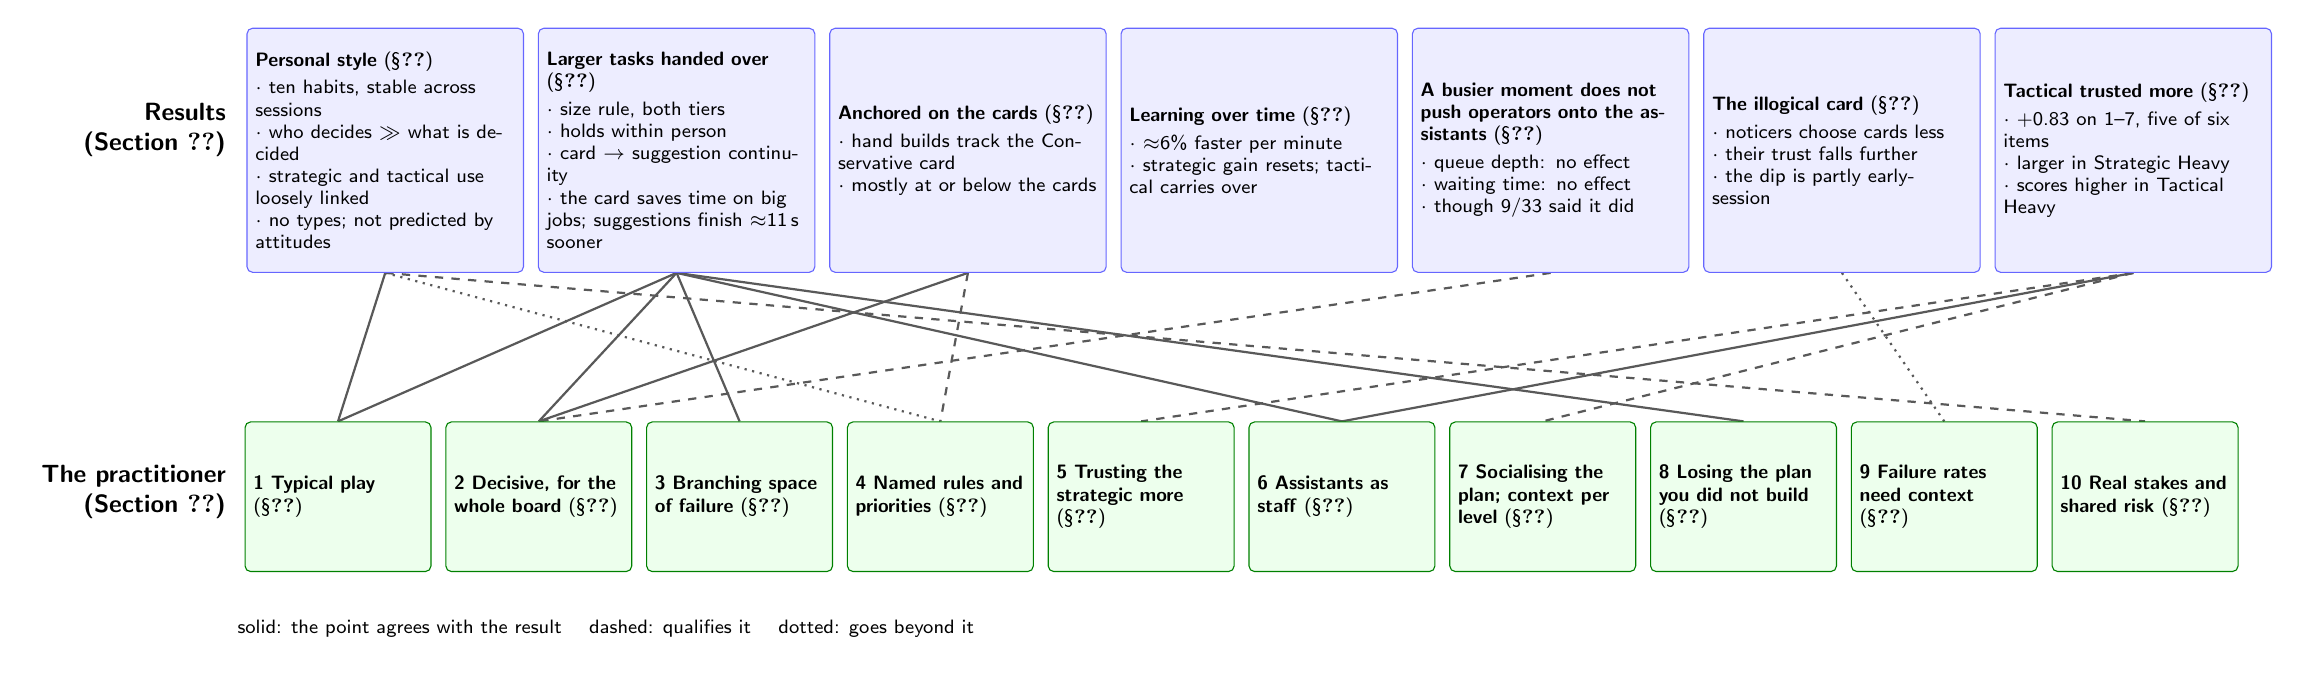
\begin{tikzpicture}[lmfont]
\lmrows
\begin{pgfonlayer}{background}\lmlinks\end{pgfonlayer}
\node[anchor=north west, font=\sffamily\scriptsize] at (-2.0,-7.4)
  {solid: the point agrees with the result \quad dashed: qualifies it \quad dotted: goes beyond it};
\end{tikzpicture}}
\caption{{\color{blue}\textbf{How the practitioner's points bear on the results.} Top: the main findings of Section~\ref{sec:results}, with their sub-findings. Bottom: the practitioner's ten points (Section~\ref{sec:qual:practitioner}). Each line is a link drawn in that section.}}
\label{fig:links-map}
\end{figure}
\end{landscape}

%% ===================================================================== Figure B
\begin{landscape}
\begin{figure}[p]
\centering
\resizebox{\linewidth}{!}{%
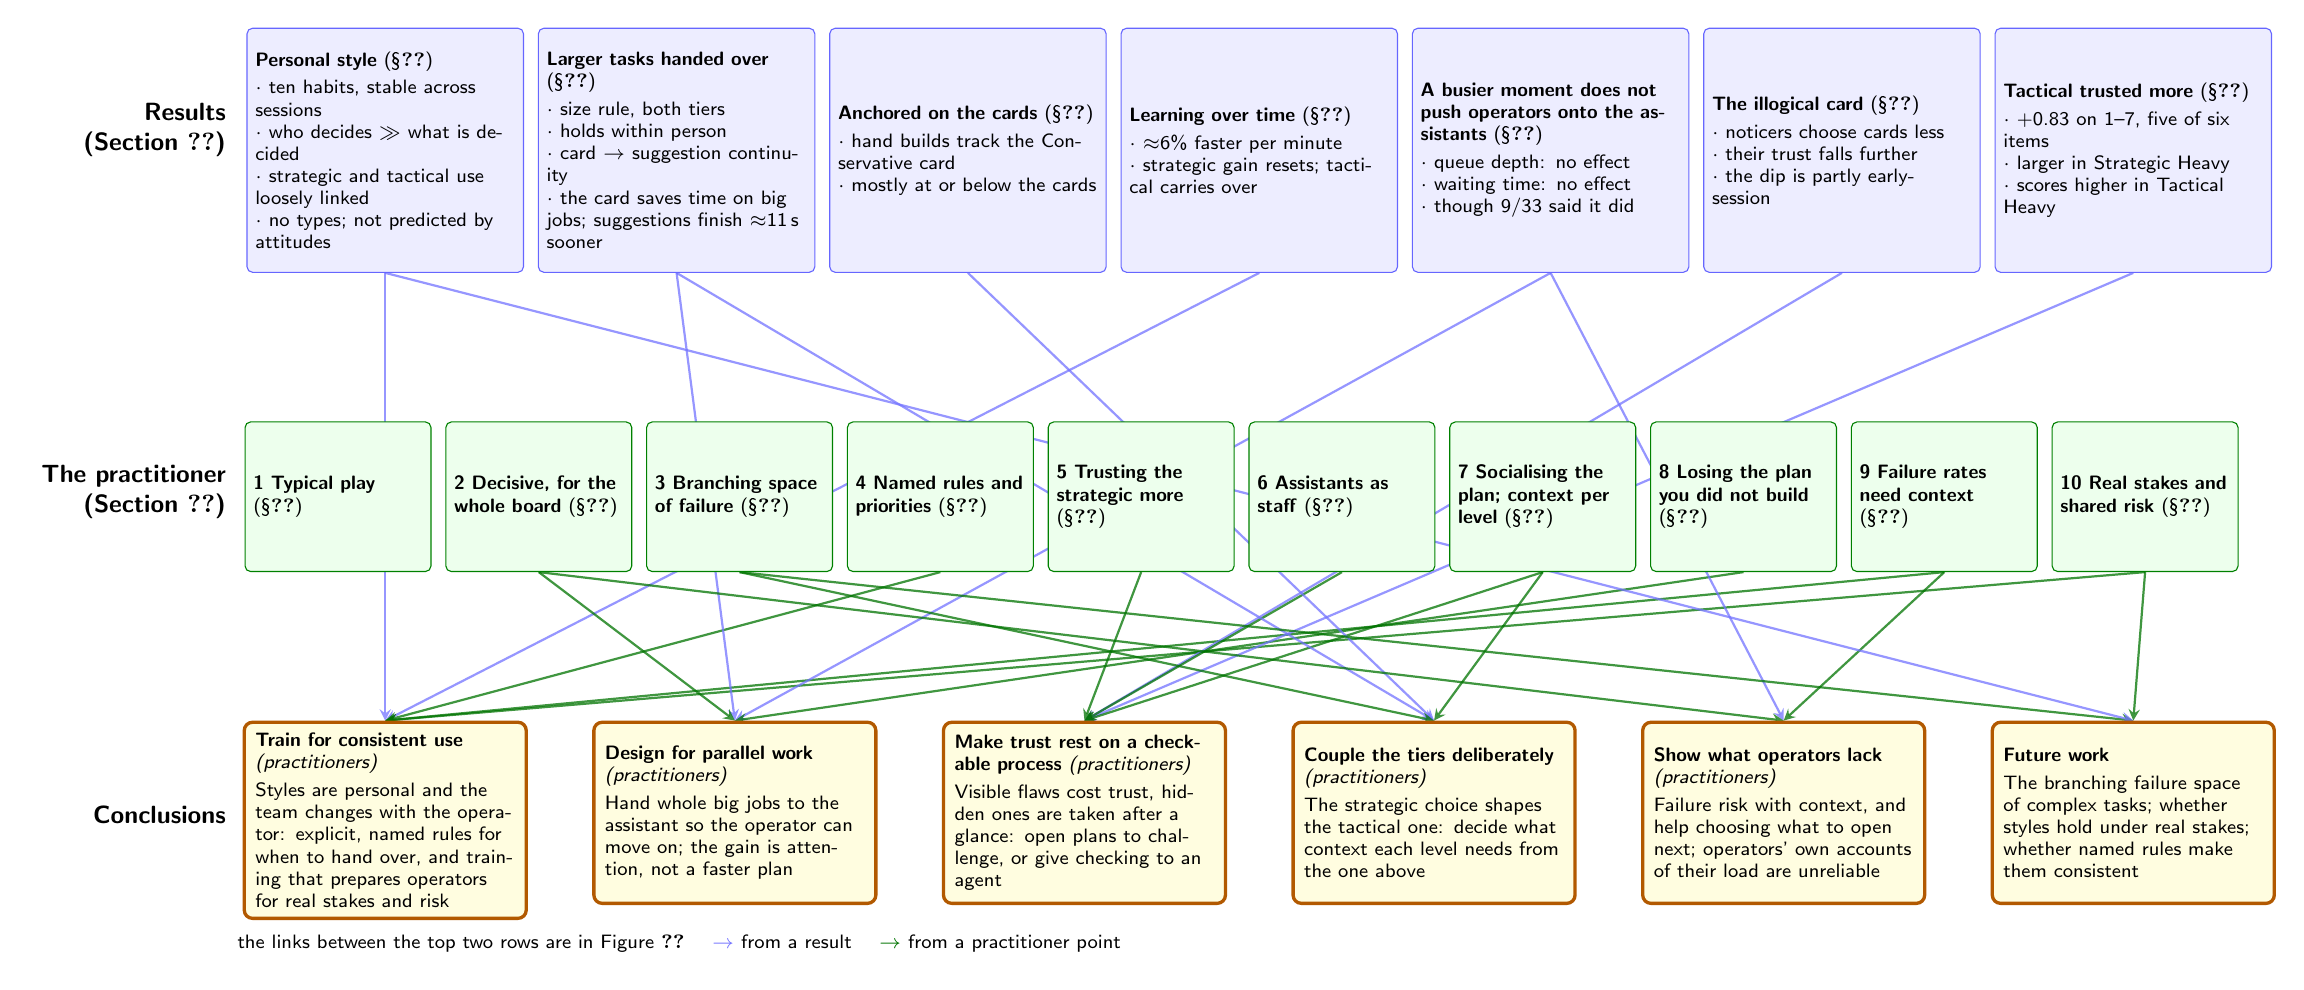
\begin{tikzpicture}[lmfont]
\lmrows
\node[rowlab] at (-1.9,-10.0) {Conclusions};
\node[con] (C1) at (0,-8.8)    {\textbf{Train for consistent use} \textit{(practitioners)}\\[2pt]Styles are personal and the team changes with the operator: explicit, named rules for when to hand over, and training that prepares operators for real stakes and risk};
\node[con] (C2) at (4.44,-8.8)  {\textbf{Design for parallel work} \textit{(practitioners)}\\[2pt]Hand whole big jobs to the assistant so the operator can move on; the gain is attention, not a faster plan};
\node[con] (C3) at (8.88,-8.8)  {\textbf{Make trust rest on a checkable process} \textit{(practitioners)}\\[2pt]Visible flaws cost trust, hidden ones are taken after a glance: open plans to challenge, or give checking to an agent};
\node[con] (C4) at (13.32,-8.8) {\textbf{Couple the tiers deliberately} \textit{(practitioners)}\\[2pt]The strategic choice shapes the tactical one: decide what context each level needs from the one above};
\node[con] (C5) at (17.76,-8.8) {\textbf{Show what operators lack} \textit{(practitioners)}\\[2pt]Failure risk with context, and help choosing what to open next; operators' own accounts of their load are unreliable};
\node[con] (C6) at (22.2,-8.8) {\textbf{Future work}\\[2pt]The branching failure space of complex tasks; whether styles hold under real stakes; whether named rules make them consistent};
\begin{pgfonlayer}{background}
  % results -> conclusions (blue) and practitioner -> conclusions (green)
  \draw[toc, blue!55] (R1.south) -- (C1.north);
  \draw[toc, blue!55] (R4.south) -- (C1.north);
  \draw[toc, green!45!black] (P4.south) -- (C1.north);
  \draw[toc, green!45!black] (P9.south) -- (C1.north);
  \draw[toc, green!45!black] (P10.south) -- (C1.north);
  \draw[toc, blue!55] (R2.south) -- (C2.north);
  \draw[toc, blue!55] (R5.south) -- (C2.north);
  \draw[toc, green!45!black] (P2.south) -- (C2.north);
  \draw[toc, green!45!black] (P8.south) -- (C2.north);
  \draw[toc, blue!55] (R6.south) -- (C3.north);
  \draw[toc, blue!55] (R7.south) -- (C3.north);
  \draw[toc, green!45!black] (P6.south) -- (C3.north);
  \draw[toc, green!45!black] (P7.south) -- (C3.north);
  \draw[toc, green!45!black] (P5.south) -- (C3.north);
  \draw[toc, blue!55] (R2.south) -- (C4.north);
  \draw[toc, blue!55] (R3.south) -- (C4.north);
  \draw[toc, green!45!black] (P3.south) -- (C4.north);
  \draw[toc, green!45!black] (P7.south) -- (C4.north);
  \draw[toc, blue!55] (R5.south) -- (C5.north);
  \draw[toc, green!45!black] (P9.south) -- (C5.north);
  \draw[toc, green!45!black] (P2.south) -- (C5.north);
  \draw[toc, green!45!black] (P3.south) -- (C6.north);
  \draw[toc, green!45!black] (P10.south) -- (C6.north);
  \draw[toc, blue!55] (R1.south) -- (C6.north);
\end{pgfonlayer}
\node[anchor=north west, font=\sffamily\scriptsize] at (-2.0,-11.4)
  {the links between the top two rows are in Figure~\ref{fig:links-map} \quad \textcolor{blue!55}{$\rightarrow$} from a result \quad \textcolor{green!45!black}{$\rightarrow$} from a practitioner point};
\end{tikzpicture}}
\caption{{\color{blue}\textbf{From results and the practitioner's reading to conclusions (draft).} The two rows of Figure~\ref{fig:links-map}, each feeding the conclusions for practitioners and for future work.}}
\label{fig:conclusions-map}
\end{figure}
\end{landscape}
